
\begin{figure}[H]	
\graphicspath{ {images/} }
    	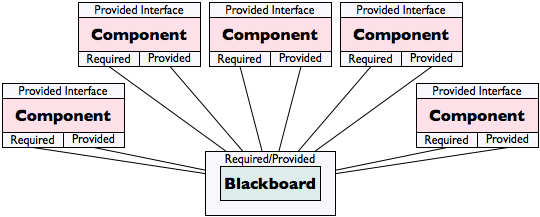
\includegraphics[scale=0.5]{bbp.png}
    	\caption{Blackboard pattern }
	\end{figure}
\subsection*{Blackboard pattern} 
To archive scalability, blackboard multiple processes to work closer together on separate threads, introduction of this pattern will help out multiple process of the buzz system to run efficiently as the pattern emphasizes multiple process working together


\begin{figure}[H]	
\graphicspath{ {images/} }
    	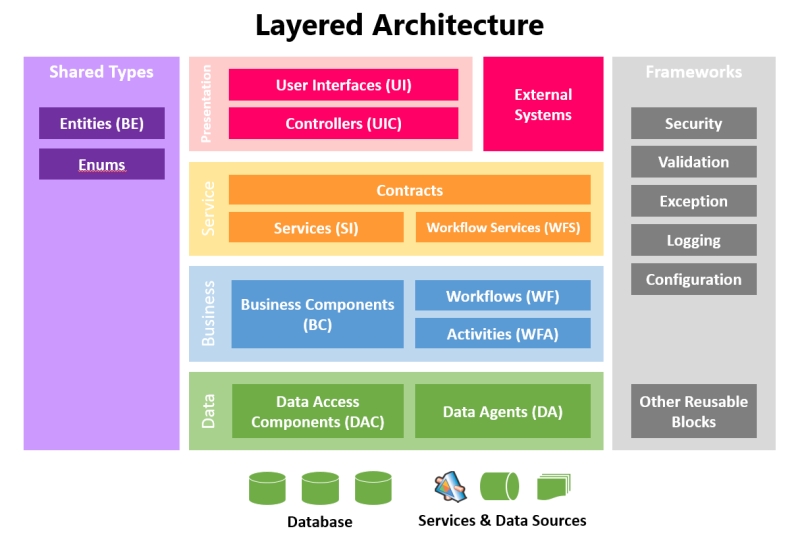
\includegraphics[scale=0.5]{layered.png}
    	\caption{Layered Architecture }
	\end{figure}
\subsection*{Layered Architecture}

System will be separated through layers; there will be User Interface  layer, services layer and process layer which includes Business logic and data. User Interface layer will handle interaction like receiving input from users, the service layer will provide the human layer with services like opening a buzz space and commenting on the buzz thread and lastly process layer will process services rendered for authorization and quality check like plagiarism. Separation through layers will enhance performance, manageability and reusability.

\begin{figure}[H]	
\graphicspath{ {images/} }
    	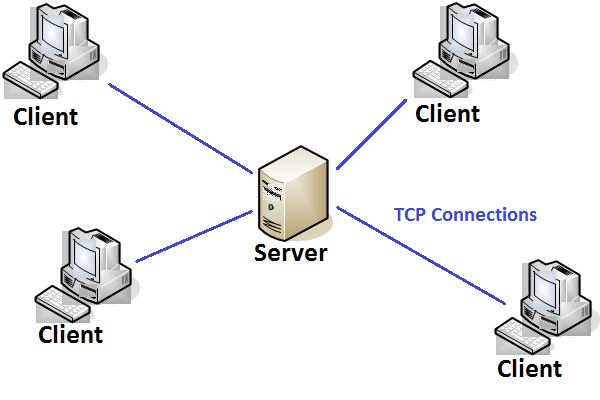
\includegraphics[scale=0.5]{csp.png}
    	\caption{Client/Server}
	\end{figure}
	
\subsection*{Client/Server} 
For communication of the server which is buzz system with users, this pattern have benefits of security as all data will be stored on the buzz system server and ease of maintenance as server is responsible of repair with client knowing of damage.

\begin{figure}[H]
	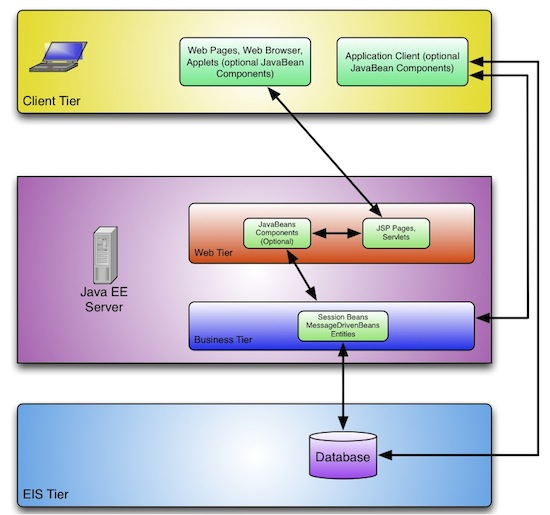
\includegraphics[scale=0.5]{MVC.jpg}
   	\caption{Java-EE system architecture}.
\end{figure}
